% ======================================================================
%  FYS4480/FYS9480  Quantum mechanics for many-particle systems
%  Week 44, October 29-30, 2026
%  Lecture slides (Beamer).  Thursday: 2 x 45 min,  Friday: 2 x 45 min.
%
%  Sources: ManyBodyPerturbationTheory.tex (the lecture transcription of
%  October 24/30/31, all of it), chapter9.tex sections 9.1-9.6 (exact
%  starting point, projection and resolvent, Brillouin-Wigner,
%  Rayleigh-Schroedinger, the two-level benchmark, the second order from
%  Wick's theorem).  Lecture 4 lists every contribution to the energy
%  through fourth order and to the wave operator through third order.
%  Exercises: Exercises/ExercisesWeek44.tex, reproduced on the last two
%  frames.  Diagram rules and their derivation: week 45.
%  Figure: ../BookFigures/chapter09/mbpt_fig01 (compile from WeeklySlides/).
%  Companion program: BookPrograms/chapter09/mbpt.py; notebook week44.ipynb.
%
%  Slide discipline: one claim per frame, the equation or table that
%  carries it, and a few short bullets.  Preamble and box macros as in
%  week43.tex.
%
%  Build:  pdflatex week44.tex  (twice)
%  Handout (no overlays):  replace \documentclass[...] by
%           \documentclass[handout,aspectratio=169]{beamer}
% ======================================================================
\documentclass[aspectratio=169,10pt]{beamer}

% ---------------------------------------------------------------- packages
\usepackage[utf8]{inputenc}
\usepackage[T1]{fontenc}
\usepackage{amsmath,amssymb,bm,mathtools}
\usepackage{booktabs}
\usepackage[most]{tcolorbox}
\usepackage{listings}
\usepackage{hyperref}
\usepackage{tikz}
\usetikzlibrary{positioning,arrows.meta,decorations.markings,shapes.misc}
\usetikzlibrary{tikzmark}

% ---------------------------------------------------------------- look
\usetheme{default}
\useinnertheme{rectangles}
\setbeamertemplate{navigation symbols}{}
\definecolor{uioblue}{RGB}{18,52,86}
\definecolor{teal}{RGB}{0,128,128}
\definecolor{warm}{RGB}{181,73,36}
\definecolor{paleblue}{RGB}{232,240,248}
\definecolor{paleteal}{RGB}{228,244,244}
\definecolor{palewarm}{RGB}{252,238,230}
\definecolor{palegreen}{RGB}{232,244,234}
\setbeamercolor{structure}{fg=uioblue}
\setbeamercolor{title}{fg=uioblue}
\setbeamercolor{frametitle}{fg=uioblue,bg=white}
\setbeamercolor{section in toc}{fg=uioblue}
\setbeamercolor{alerted text}{fg=warm}
\setbeamercolor{block title}{fg=white,bg=uioblue}
\setbeamercolor{block body}{bg=paleblue}
\setbeamercolor{block title example}{fg=white,bg=teal}
\setbeamercolor{block body example}{bg=paleteal}
\setbeamerfont{frametitle}{size=\large,series=\bfseries}
\setbeamerfont{title}{size=\LARGE,series=\bfseries}
\setbeamertemplate{frametitle}{%
  \vspace*{0.6em}\insertframetitle\par
  \vspace*{-0.2em}{\color{teal}\rule{\textwidth}{0.6pt}}}
\setbeamertemplate{footline}{%
  \hbox{\begin{beamercolorbox}[wd=\paperwidth,ht=2.4ex,dp=1.2ex,leftskip=1em,rightskip=1em]{structure}%
  \footnotesize FYS4480/9480 -- Week 44 \hfill \insertsection \hfill \insertframenumber/\inserttotalframenumber
  \end{beamercolorbox}}}
\setbeamertemplate{itemize items}[circle]
\setbeamertemplate{enumerate items}[default]
\setbeamertemplate{section page}{%
  \begin{centering}
    {\usebeamerfont{section title}\usebeamercolor[fg]{title}\LARGE\bfseries\insertsection\par}
    \vspace{0.5em}{\color{teal}\rule{0.5\textwidth}{1pt}}
  \end{centering}}
\AtBeginSection[]{\frame{\sectionpage}}

% ---------------------------------------------------------------- boxes
\newcounter{thinkctr}
\newcommand{\thinkq}[2]{%
  \stepcounter{thinkctr}%
  \vfill
  \begin{tcolorbox}[enhanced,colback=palewarm,colframe=warm,boxrule=1.2pt,arc=4pt,
    grow to left by=6mm,grow to right by=6mm,
    left=16pt,right=16pt,top=16pt,bottom=18pt,
    fonttitle=\bfseries\Large,fontupper=\Large,
    title={Pause to think \#\thethinkctr\hfill\mdseries\normalsize(about #1 min -- discuss with your neighbour)}]
  #2
  \end{tcolorbox}
  \vfill}
\newcommand{\thinka}[1]{%
  \vfill
  \begin{tcolorbox}[enhanced,colback=paleteal,colframe=teal,boxrule=1.2pt,arc=4pt,
    grow to left by=6mm,grow to right by=6mm,
    left=16pt,right=16pt,top=16pt,bottom=18pt,
    fonttitle=\bfseries\Large,fontupper=\large,
    title={Answer to pause \#\thethinkctr}]
  #1
  \end{tcolorbox}
  \vfill}
\newcommand{\mbbox}[1]{%
  \begin{tcolorbox}[colback=paleblue,colframe=uioblue,title={\bfseries Many-body connection}]
  #1
  \end{tcolorbox}}
\newcommand{\warnbox}[1]{%
  \begin{tcolorbox}[colback=palewarm,colframe=warm,title={\bfseries A trap to avoid}]
  #1
  \end{tcolorbox}}
\newcommand{\numbox}[1]{%
  \begin{tcolorbox}[colback=palegreen,colframe=teal!70!black,title={\bfseries Measured}]
  #1
  \end{tcolorbox}}

% ---------------------------------------------------------------- code
\lstset{language=Python,basicstyle=\ttfamily\scriptsize,
  keywordstyle=\color{uioblue}\bfseries,commentstyle=\color{teal},
  stringstyle=\color{warm},showstringspaces=false,columns=fullflexible,
  frame=single,rulecolor=\color{paleblue},backgroundcolor=\color{white},
  breaklines=true}

% ---------------------------------------------------------------- macros
\newcommand{\ket}[1]{\vert #1\rangle}
\newcommand{\bra}[1]{\langle #1\vert}
\newcommand{\braket}[2]{\langle #1\vert #2\rangle}
\newcommand{\element}[3]{\langle #1\vert #2\vert #3\rangle}
\DeclareMathOperator{\tr}{tr}
\newcommand{\bigO}{\mathcal{O}}
\newcommand{\bmat}[1]{\bm{#1}}
\newcommand{\Amat}[1]{\bm{A}^{#1}}
\newcommand{\Bmat}[1]{\bm{B}^{#1}}
\newcommand{\hH}{\hat{H}}
\newcommand{\ad}[1]{a_{#1}^{\dagger}}
\newcommand{\ketbra}[2]{\vert #1\rangle\langle #2\vert}
% normal ordering with respect to the reference determinant |c> (as in week 40)
\newcommand{\nc}[1]{\bigl\{#1\bigr\}}

% ---------------------------------------------------------------- diagrams
\tikzset{
  tens/.style={draw=uioblue,fill=paleblue,thick,rounded corners=1pt,minimum size=7mm,font=\small},
  mpo/.style={draw=warm,fill=palewarm,thick,rounded corners=1pt,minimum size=7mm,font=\small},
  env/.style={draw=teal!70!black,fill=paleteal,thick,rounded corners=1pt,
              minimum width=7mm,minimum height=14mm,font=\small},
  leg/.style={thick,uioblue},
  dlab/.style={font=\scriptsize},
  every picture/.style={scale=0.8,baseline=(current bounding box.center)}
}

\graphicspath{{../BookFigures/}{./}}

\newcommand{\dd}{\mathrm{d}}


% ---------------------------------------------------------------- MBPT macros
\newcommand{\mel}[3]{\langle #1\lvert #2\rvert #3\rangle}
\newcommand{\av}[1]{\langle #1\rangle_0}
\newcommand{\cre}[1]{a_{#1}^{\dagger}}
\newcommand{\ann}[1]{a_{#1}}
\newcommand{\no}[1]{\bigl\{#1\bigr\}}
\newcommand{\vbar}[4]{\overline v_{#1#2#3#4}}
\newcommand{\Eref}{E_{\mathrm{ref}}}
\newcommand{\ph}{\Phi_0}
\newcommand{\Psizero}{\Psi_0}
\newcommand{\ord}[1]{\mathcal O(#1)}
\newcommand{\Rzero}{R_0}
\tikzset{fermion/.style={line width=.8pt,uioblue,postaction={decorate},decoration={markings,mark=at position .56 with {\arrow{Stealth}}}},
  interaction/.style={dashed,line width=.8pt,warm},
  vertex/.style={circle,fill=warm,inner sep=1.7pt}}
\newcommand{\wickpattern}[1]{%
\begin{tikzpicture}[x=.86cm,y=.72cm,every node/.style={font=\small,inner sep=1.3pt},scale=1,baseline=(current bounding box.center)]
\node(p)at(0,0){\(\cre{p}\)};\node(q)at(1,0){\(\cre{q}\)};
\node(s)at(2,0){\(\ann{s}\)};\node(r)at(3,0){\(\ann{r}\)};
\node(a)at(4,0){\(\cre{a}\)};\node(b)at(5,0){\(\cre{b}\)};
\node(j)at(6,0){\(\ann{j}\)};\node(i)at(7,0){\(\ann{i}\)};
\draw[uioblue,line width=.6pt,rounded corners=3pt](p.north)--++(0,1.05)-|(i.north);
\draw[uioblue,line width=.6pt,rounded corners=3pt](q.north)--++(0,.64)-|(j.north);
\ifnum#1=1\relax
\draw[teal,line width=.7pt,rounded corners=3pt](s.south)--++(0,-.9)-|(b.south);
\draw[teal,line width=.7pt,rounded corners=3pt](r.south)--++(0,-.48)-|(a.south);
\else
\draw[teal,line width=.7pt,rounded corners=3pt](s.south)--++(0,-.9)-|(a.south);
\draw[teal,line width=.7pt,rounded corners=3pt](r.south)--++(0,-.48)-|(b.south);
\fi
\end{tikzpicture}}

% ---------------------------------------------------------------- title
\title{Many-body perturbation theory: reference states, projection methods and energy corrections}
\subtitle{FYS4480/FYS9480 -- Week 44, October 29--30, 2026}
\author{Cecilie Glittum and Morten Hjorth-Jensen}
\institute{Department of Physics,\\
University of Oslo, Norway}
\date{}

\begin{document}

\begin{frame}[plain]
  \vspace*{-0.2em}{\setbeamerfont{title}{size=\Large,series=\bfseries}\titlepage}
  \vfill
  \begin{center}\small
  Thursday: a reference determinant and its excitations, the exact energy projected onto it, projection operators and the reduced resolvent, Brillouin-Wigner versus Rayleigh-Schr\"odinger, and the first three orders\\
  Friday: the second-order energy from Wick's theorem, a two-level benchmark through fourth order, and every contribution to the energy through fourth order and to the wave operator through third\\[0.8em]
  {\footnotesize Reading: lecture notes chapter 9, sections 9.1--9.6; Shavitt and Bartlett, chapter 2; Szabo and Ostlund, chapter 6. Code: \texttt{BookPrograms/chapter09/mbpt.py}; notebook \texttt{week44.ipynb}.\\[0.2em]
  Exercises: Last two slides; answers on the week-45 slides.}
  \end{center}
\end{frame}

\begin{frame}[shrink=5]{Plan for week 44}
  \begin{block}{Thursday, $2\times45$ min: reference states, projection methods and systematic orders (sections 9.1--9.4)}
    \begin{itemize}
      \item A reference determinant, its $1p1h$ and $2p2h$ excitations, and the exact energy projected onto the reference: only singles and doubles couple directly
      \item A two-state problem solved by hand: the orders we must recover
      \item Intermediate normalisation, two energy differences that must be kept apart, $P$ and $Q$, the reduced resolvent, an exact equation for $Q\ket{\Psizero}$ and its Neumann series
      \item Two choices of starting energy: Brillouin-Wigner ($\omega=E_0$, implicit) and Rayleigh-Schr\"odinger ($\omega=\varepsilon_0$, explicit)
      \item A resolvent identity, the resummation in $Q$ space, the energy-dependent effective Hamiltonian, and the secular equation recovered
      \item Rayleigh-Schr\"odinger order by order: $E^{(1)}$, $E^{(2)}$, and the normalisation subtraction in $E^{(3)}$
    \end{itemize}
  \end{block}
  \begin{block}{Friday, $2\times45$ min: the second-order energy and a fourth-order check (sections 9.5--9.6)}
    \begin{itemize}
      \item First-order direct and exchange terms; which intermediate determinants contribute; the perturbation normal-ordered, $H_I=E^{(1)}+U_N+V_N$
      \item Singles: the coherent mean-field sum. Doubles: Wick contractions, the counting factor, the leading amplitude. The complete $E^{(2)}$
      \item A purely off-diagonal two-level benchmark: Brillouin-Wigner exact with two vertices, Rayleigh-Schr\"odinger through fourth order, only the folded term survives
      \item \alert{The list}: every contribution to the energy through fourth order and to the wave operator through third order
    \end{itemize}
  \end{block}
\end{frame}

\begin{frame}[shrink=12]{Where we are, and the route through this week}
  \begin{columns}[T]
    \column{0.5\textwidth}
    \begin{block}{Done}
      \begin{itemize}
        \item Full CI (weeks 37--38): exact, exponential
        \item Hartree-Fock (weeks 38--39): the best single determinant, $f_{ai}=0$
        \item Stability, DMRG, the electron gas, density functional theory (weeks 39--43)
      \end{itemize}
    \end{block}
    \column{0.5\textwidth}
    \begin{block}{This week}
      \begin{enumerate}
        \item Reference determinants and perturbative amplitudes
        \item Projection operators and the reduced resolvent
        \item Brillouin-Wigner and Rayleigh-Schr\"odinger expansions
        \item Second-order energy from single and double excitations
        \item A two-level check through fourth order
      \end{enumerate}
    \end{block}
  \end{columns}
  \vspace{0.6em}
  \mbbox{Scope: nondegenerate, time-independent perturbation theory, with a single reference determinant and a Hamiltonian containing at most two-body terms. Next week the same terms are drawn as diagrams, and the rules for reading them off are derived.}
\end{frame}

% ======================================================================
\section{Thursday, lecture 1: Reference states and expansions}
% ======================================================================

\begin{frame}{A reference determinant and its excitations (section 9.1)}
Choose an orthonormal determinant basis built on \(\ket{\ph}\):
\[
\ket{\Psizero}=\ket{\ph}
+\sum_{ia}c_i^a\ket{\Phi_i^a}
+\sum_{\substack{i<j\\a<b}}c_{ij}^{ab}\ket{\Phi_{ij}^{ab}}
+\cdots ,
\qquad
\ket{\Phi_i^a}=\cre{a}\ann{i}\ket{\ph},\qquad
\ket{\Phi_{ij}^{ab}}=\cre{a}\cre{b}\ann{j}\ann{i}\ket{\ph}.
\]
\begin{itemize}
\item \(i,j,k,\ldots\): occupied orbitals; \(a,b,c,\ldots\): unoccupied orbitals (weeks 37--38).
\item The exact expansion reaches all allowed \(NpNh\) excitations.
\item MBPT approximates the amplitudes order by order.
\end{itemize}
\smallskip
\small Here the reference coefficient is one; doubles are summed once, with \(i<j\) and \(a<b\).
\end{frame}

\begin{frame}{Projecting the energy onto the reference}
With \(\braket{\ph}{\Psizero}=1\) and \(H\ket{\Psizero}=E_0\ket{\Psizero}\),
\[
E_0=\mel{\ph}{H}{\Psizero},\qquad
\Eref=\mel{\ph}{H}{\ph}.
\]
For an at-most-two-body Hamiltonian,
\[
\boxed{E_0-\Eref
=\sum_{ia}c_i^a f_{ia}
+\sum_{\substack{i<j\\a<b}}c_{ij}^{ab}\vbar{i}{j}{a}{b}.}
\qquad
f_{ia}\equiv\mel{\ph}{H}{\Phi_i^a},\quad
\vbar{i}{j}{a}{b}\equiv\langle ij\lvert v\rvert ab\rangle_{\!\rm AS}.
\]
\begin{itemize}
\item Only singles and doubles couple directly to the reference (the energy equation of week 38).
\item Higher excitations still influence the exact amplitudes.
\end{itemize}
\end{frame}

\begin{frame}{Preview: leading amplitudes and second-order energy}
For \(H_0=\sum_p\varepsilon_p\cre{p}\ann{p}\), with \(\varepsilon_0=\sum_{i\in\mathrm{occ}}\varepsilon_i\), the leading amplitudes will turn out to be
\[
c_i^{a(1)}=\frac{f_{ai}}{\varepsilon_i-\varepsilon_a},\qquad
c_{ij}^{ab(1)}=\frac{\vbar{a}{b}{i}{j}}
 {\varepsilon_i+\varepsilon_j-\varepsilon_a-\varepsilon_b}.
\]
Substitution into the projected energy gives
\[
E^{(2)}=
\sum_{ia}\frac{|f_{ai}|^2}{\varepsilon_i-\varepsilon_a}
+\sum_{\substack{i<j\\a<b}}
\frac{|\vbar{a}{b}{i}{j}|^2}
 {\varepsilon_i+\varepsilon_j-\varepsilon_a-\varepsilon_b}.
\]
\begin{exampleblock}{Hartree-Fock reference}
For canonical Hartree-Fock orbitals, \(f_{ai}=0\) (Brillouin, week 38): the singles term vanishes. This is a special case, not a condition on a general reference.
\end{exampleblock}
\end{frame}

\begin{frame}{A two-state illustration of the perturbative idea}
Use a one-particle model to make the algebra transparent:
\[
H=H_0+H_I,\qquad
H_0=\sum_{p=1}^{2}\varepsilon_p\cre{p}\ann{p},\qquad
H_I=g\sum_{p,q=1}^{2}\cre{p}\ann{q},
\]
with \(\varepsilon_1<\varepsilon_2\) and \(\ket{p}=\cre{p}\ket{0}\).
\[
\braket{p}{q}=\delta_{pq},\qquad
P=\ket{1}\bra{1},\qquad Q=\ket{2}\bra{2},\qquad P+Q=1.
\]
For example,
\[
\mel{1}{H_I}{2}
=g\sum_{pq}\mel{0}{\ann{1}\cre{p}\ann{q}\cre{2}}{0}
=g\sum_{pq}\delta_{1p}\delta_{q2}=g.
\]
\small This is an algebraic benchmark inside the many-body development; it is not an interacting many-particle system.
\end{frame}

\begin{frame}{Exact eigenvalues of the two-state model}
In the basis \(\{\ket{1},\ket{2}\}\),
\[
H=\begin{pmatrix}\varepsilon_1+g&g\\g&\varepsilon_2+g\end{pmatrix},
\qquad \det(H-EI)=0,
\qquad
E_\pm=\frac{\varepsilon_1+\varepsilon_2}{2}+g
\pm\sqrt{\frac{(\varepsilon_2-\varepsilon_1)^2}{4}+g^2}.
\]
Define the positive gap \(\Delta=\varepsilon_2-\varepsilon_1>0\). Then
\[
\boxed{E_-=\varepsilon_1+g+
\frac{\Delta}{2}\left[1-\sqrt{1+\frac{4g^2}{\Delta^2}}\right].}
\]
\small The positive gap fixes the branch and the signs before expanding the square root.
\end{frame}

\begin{frame}{Reading off perturbative orders}
Use
\(\sqrt{1+x}=1+\frac{x}{2}-\frac{x^2}{8}+\cdots\) with \(x=4g^2/\Delta^2\). The lower eigenvalue becomes
\[
\boxed{E_-=\varepsilon_1+g-\frac{g^2}{\Delta}
+\frac{g^4}{\Delta^3}+\ord{g^6}.}
\]
\begin{center}
\begin{tabular}{ccccc}
\toprule
Unperturbed & First order & Second order & Third order & Fourth order\\
\midrule
\(\varepsilon_1\) & \(g\) & \(-g^2/\Delta\) & \(0\) & \(g^4/\Delta^3\)\\
\bottomrule
\end{tabular}
\end{center}
\begin{block}{The task of perturbation theory}
Recover these contributions from the Hamiltonian and the reference state, without solving the full eigenvalue problem first.
\end{block}
\end{frame}

\begin{frame}{Formal MBPT and intermediate normalisation (section 9.1)}
\[
H=H_0+H_I,\qquad H_0\ket{\Phi_m}=\varepsilon_m\ket{\Phi_m},
\qquad H\ket{\Psizero}=E_0\ket{\Psizero}.
\]
Assume a nondegenerate reference \(\ket{\ph}\) with nonzero overlap with the exact state.
\[
\braket{\ph}{\ph}=1,\qquad
\boxed{\braket{\ph}{\Psizero}=1},\qquad
\ket{\Psizero}=\ket{\ph}+\sum_{m\ne0}c_m\ket{\Phi_m}.
\]
\begin{itemize}
\item The reference coefficient is fixed to one.
\item Intermediate normalisation does not require \(\braket{\Psizero}{\Psizero}=1\).
\item All excited determinants are included in the label \(m\ne0\).
\end{itemize}
\end{frame}

\begin{frame}{Pause to think \#1}
\thinkq{3}{Intermediate normalisation sets \(\braket{\ph}{\Psizero}=1\) instead of \(\braket{\Psizero}{\Psizero}=1\).
\begin{enumerate}
\item Why is this a convenience and not an approximation?
\item Which assumption about \(\ket{\ph}\) is needed for it to be possible at all?
\item The exact energy is \(E_0=\mel{\ph}{H}{\Psizero}\). Is this an expectation value? Is it an upper bound?
\end{enumerate}}
\end{frame}

\begin{frame}{Answer to pause \#1}
\thinka{%
\begin{enumerate}
\item The Schr\"odinger equation is linear: any multiple of \(\ket{\Psizero}\) is a solution with the same energy. Choosing the multiple such that the reference coefficient is one changes the norm, not the physics; the normalised state is \(\ket{\Psizero}/\sqrt{\braket{\Psizero}{\Psizero}}\).
\item \(\braket{\ph}{\Psizero}\ne0\): the reference must have a non-zero component along the exact ground state. If it does not -- wrong symmetry, wrong particle number, or a reference that is orthogonal to the target -- no rescaling can produce the coefficient one.
\item It is a \emph{transition} matrix element, not an expectation value \(\mel{\Psizero}{H}{\Psizero}/\braket{\Psizero}{\Psizero}\). The two agree only for the exact state; for an approximate \(\ket{\Psizero}\) the projected energy is \emph{not} variational and can lie below \(E_0\). This is why perturbation theory can cross the exact answer from either side.
\end{enumerate}}
\end{frame}

\begin{frame}{Two energy differences that must be distinguished}
Reference projection gives
\[
E_0=\varepsilon_0+\mel{\ph}{H_I}{\Psizero},\qquad
E^{(1)}=\mel{\ph}{H_I}{\ph},
\qquad
\Eref=\mel{\ph}{H}{\ph}=\varepsilon_0+E^{(1)}.
\]
\begin{block}{Energy shift relative to the unperturbed state}
\[\Delta E\equiv E_0-\varepsilon_0=E^{(1)}+E^{(2)}+\cdots.\]
\end{block}
\begin{exampleblock}{Correlation energy relative to the reference determinant}
\[E_0-\Eref=E^{(2)}+E^{(3)}+\cdots.\]
\end{exampleblock}
\small The first-order term is the mean-field energy of the reference, not correlation; whether it vanishes depends on the partition. Correlation begins at second order.
\end{frame}

\begin{frame}{Separating the reference and its complement (section 9.2)}
\[
P=\ket{\ph}\bra{\ph},\qquad
Q=\sum_{m\ne0}\ket{\Phi_m}\bra{\Phi_m},
\]
\[
P^2=P,\quad Q^2=Q,\quad P+Q=1,\quad PQ=QP=0,
\qquad
[P,H_0]=[Q,H_0]=0.
\]
Intermediate normalisation implies
\[
P\ket{\Psizero}=\ket{\ph},\qquad
\boxed{\ket{\Psizero}=\ket{\ph}+Q\ket{\Psizero}.}
\]
\begin{itemize}
\item \(P\): one-dimensional model space.
\item \(Q\): all configurations excited from the reference.
\end{itemize}
\end{frame}

\begin{frame}{The reduced resolvent}
For a scalar starting energy \(\omega\), define
\[
\boxed{R_Q(\omega)\equiv Q(\omega-H_0)^{-1}Q
=\sum_{m\ne0}\frac{\ket{\Phi_m}\bra{\Phi_m}}
 {\omega-\varepsilon_m}.}
\]
\[
R_Q(\omega)\ket{\ph}=0,\qquad
R_Q(\omega)\ket{\Phi_m}=
\frac{\ket{\Phi_m}}{\omega-\varepsilon_m}\quad(m\ne0).
\]
\begin{block}{The inverse is restricted to \(Q\) space}
At \(\omega=\varepsilon_0\), the full inverse has a reference-state pole. The reduced resolvent remains defined if \(\varepsilon_0\ne\varepsilon_m\) for all \(m\ne0\) -- this is where non-degeneracy is used.
\end{block}
\end{frame}

\begin{frame}{An exact equation for the correlated component}
Rewrite the Schr\"odinger equation as
\[
(\omega-H_0)\ket{\Psizero}=(\omega-E_0+H_I)\ket{\Psizero}.
\]
Project and apply the reduced inverse:
\[
Q\ket{\Psizero}=R_Q(\omega)(\omega-E_0+H_I)\ket{\Psizero},
\qquad
\boxed{\ket{\Psizero}=\ket{\ph}
+R_Q(\omega)(\omega-E_0+H_I)\ket{\Psizero}.}
\]
\begin{itemize}
\item The Hamiltonian and reference are known.
\item The exact energy \(E_0\) and correlated state are still unknown: exact, and useless as it stands.
\end{itemize}
\end{frame}

\begin{frame}{Iterating the wave-function equation}
Set \(A(\omega)=R_Q(\omega)(\omega-E_0+H_I)\). Repeated substitution yields
\begin{align*}
\ket{\Psizero}&=\ket{\ph}+A\ket{\Psizero}
=\ket{\ph}+A\ket{\ph}+A^2\ket{\Psizero}
=\ket{\ph}+A\ket{\ph}+A^2\ket{\ph}+\cdots.
\end{align*}
Formally,
\[
\boxed{\ket{\Psizero}=\sum_{n=0}^{\infty}
\left[R_Q(\omega)(\omega-E_0+H_I)\right]^n\ket{\ph},}
\qquad
\Delta E=\sum_{n=0}^{\infty}
\mel{\ph}{H_I\left[R_Q(\omega)(\omega-E_0+H_I)\right]^n}{\ph}.
\]
\warnbox{This is a formal Neumann series. Its convergence is not guaranteed by the algebraic iteration alone; Friday's benchmark shows the series diverging while the exact answer stays perfectly smooth.}
\end{frame}

\begin{frame}{Two choices of starting energy (section 9.3)}
\begin{columns}[T,onlytextwidth]
\column{.48\textwidth}
\begin{block}{Brillouin-Wigner (BW)}
\[\omega=E_0.\]
The unknown exact energy enters the denominators; the equation is implicit and must be solved self-consistently.
\end{block}
\column{.48\textwidth}
\begin{exampleblock}{Rayleigh-Schr\"odinger (RS)}
\[\omega=\varepsilon_0.\]
Fixed unperturbed denominators; collect equal powers of the interaction, and expand \(\Delta E\) in the numerators too.
\end{exampleblock}
\end{columns}
\vspace{0.8em}
The first terms of the Brillouin-Wigner series, with \(\av{X}\equiv\mel{\ph}{X}{\ph}\) and \(R_E=R_Q(E_0)\):
\[
\Delta E=\av{H_I}
+\av{H_I R_E H_I}
+\av{H_I R_E H_I R_E H_I}+\cdots ,
\qquad
R_E=\sum_{m\ne0}\frac{\ket{\Phi_m}\bra{\Phi_m}}{E_0-\varepsilon_m}.
\]
\begin{itemize}
\item Terms are ordered by the number of explicit interaction vertices.
\item Because \(E_0\) itself depends on the interaction, a finite BW truncation is \emph{not} a Taylor expansion in the coupling.
\end{itemize}
\end{frame}

% ======================================================================
\section{Thursday, lecture 2: Projection methods and orders}
% ======================================================================

\begin{frame}{The projection framework in compact form}
\[
P=\ket{\ph}\bra{\ph},\qquad Q=1-P,\qquad
R_Q(\omega)=\sum_{m\ne0}\frac{\ket{\Phi_m}\bra{\Phi_m}}{\omega-\varepsilon_m},
\]
\[
\Delta E=\sum_{n=0}^{\infty}
\av{H_I\left[R_Q(\omega)(\omega-E_0+H_I)\right]^n}.
\]
Keep the two baselines explicit:
\[
\Delta E=E_0-\varepsilon_0=\mel{\ph}{H_I}{\Psizero},\qquad
E_0-\Eref=\sum_{m\ne0}c_m\mel{\ph}{H_I}{\Phi_m},\qquad
\Eref=\varepsilon_0+\mel{\ph}{H_I}{\ph}.
\]
For \(\omega=E_0\): \(\Delta E=\av{H_I}+\av{H_I R_E H_I}+\av{H_I R_E H_I R_E H_I}+\cdots\).
\begin{block}{Next step}
Sum the repeated propagation and interactions within \(Q\) space into one energy-dependent resolvent.
\end{block}
\end{frame}

\begin{frame}{A resolvent identity}
For invertible operators \(A\) and \(A-B\),
\[
\boxed{(A-B)^{-1}=A^{-1}+A^{-1}B(A-B)^{-1}.}
\]
Check by multiplying on the right by \(A-B\):
\[
\left[A^{-1}+A^{-1}B(A-B)^{-1}\right](A-B)
=1-A^{-1}B+A^{-1}B=1.
\]
Iterating gives
\[
(A-B)^{-1}=A^{-1}+A^{-1}BA^{-1}
+A^{-1}BA^{-1}BA^{-1}+\cdots .
\]
\small Preserve the order of the operator factors; \(A\) and \(B\) need not commute.
\end{frame}

\begin{frame}{Resumming propagation in the complementary space}
Take \(A=E_0-QH_0Q\) and \(B=QH_IQ\), acting within \(Q\) space. Define
\[
G_Q(E_0)=Q\left(E_0-QHQ\right)^{-1}_{Q}Q
=Q\left(E_0-H_0-QH_IQ\right)^{-1}_{Q}Q .
\]
Its formal expansion is
\[
G_Q(E_0)=R_E+R_E H_I R_E
+R_E H_I R_E H_I R_E+\cdots,
\]
where every intermediate propagation is restricted to \(Q\); the subscript \(Q\) specifies where the inverse is taken.
\mbbox{\(G_Q\) is the resolvent of the \emph{full} Hamiltonian restricted to the excited space. It is the object a Green's function approach (chapter 12) would start from.}
\end{frame}

\begin{frame}{An exact energy-dependent effective Hamiltonian}
The projected Schr\"odinger equation gives \(Q\ket{\Psizero}=G_Q(E_0)H_I\ket{\ph}\). Hence
\[
\boxed{\Delta E=\av{H_I}+\av{H_I G_Q(E_0)H_I},}
\qquad
\boxed{\ket{\Psizero}=\left[1+G_Q(E_0)H_I\right]\ket{\ph}.}
\]
Equivalently, in the model space,
\[
H_{\rm eff}(E_0)=PHP+PHQ(E_0-QHQ)^{-1}_{Q}QHP .
\]
\small These equations are exact where the reference overlap is nonzero and the required \(Q\)-space inverse exists. Their energy dependence makes them implicit (Feshbach--L\"owdin partitioning).
\end{frame}

\begin{frame}{Applying the projected resolvent to two states}
Return to
\[
H=\begin{pmatrix}\varepsilon_1+g&g\\g&\varepsilon_2+g\end{pmatrix},
\qquad P=\ket{1}\bra{1},\quad Q=\ket{2}\bra{2}.
\]
There is only one state in \(Q\):
\[
QHQ=(\varepsilon_2+g)Q,\qquad
G_Q(E_0)=\frac{\ket{2}\bra{2}}{E_0-\varepsilon_2-g},
\qquad
\mel{1}{H_I}{1}=g,\qquad
\mel{1}{H_I}{2}=\mel{2}{H_I}{1}=g.
\]
The resummed BW equation becomes
\[
E_0-\varepsilon_1=g+\frac{g^2}{E_0-\varepsilon_2-g}
\quad\Longleftrightarrow\quad
\boxed{(E_0-\varepsilon_1-g)(E_0-\varepsilon_2-g)-g^2=0,}
\]
which is precisely \(\det(H-E_0)=0\).
\begin{block}{What is exact here?}
The complete \(Q\)-space resummation plus the self-consistent solution reproduces the exact eigenvalues. This is not a claim that ordinary second-order perturbation theory is exact.
\end{block}
\end{frame}

\begin{frame}{Rayleigh-Schr\"odinger: fix the starting energy (section 9.4)}
Set \(\omega=\varepsilon_0\) and introduce
\[
R_0=\frac{Q}{\varepsilon_0-H_0},\qquad
\Delta E=E_0-\varepsilon_0 .
\]
Then
\[
\ket{\Psizero}=\ket{\ph}+R_0(H_I-\Delta E)\ket{\Psizero},
\qquad
\boxed{\Delta E=\sum_{n=0}^{\infty}
\av{H_I\left[R_0(H_I-\Delta E)\right]^n}.}
\]
\begin{itemize}
\item The denominators now involve unperturbed energies only.
\item The energy shift inside the operator product must itself be expanded.
\item \(R_0\ket{\ph}=0\) removes a rightmost scalar subtraction.
\end{itemize}
\end{frame}

\begin{frame}{Collect terms of the same perturbative order}
Introduce a bookkeeping parameter \(\eta\):
\[
H(\eta)=H_0+\eta H_I,\qquad
E_0(\eta)=\varepsilon_0+\sum_{n\ge1}\eta^nE^{(n)}.
\]
The first terms of the implicit energy equation are
\[
\Delta E=\av{H_I}
+\av{H_I R_0(H_I-\Delta E)}
+\av{H_I R_0(H_I-\Delta E)R_0H_I}+\cdots .
\]
Since \(R_0\ket{\ph}=0\),
\(\av{H_I R_0(H_I-\Delta E)}=\av{H_I R_0H_I}\).
\warnbox{Set \(\eta=1\) after collecting equal powers. A superscript \((n)\) denotes an energy contribution of order \(n\) in the interaction, \emph{not} an excitation rank: a first-order amplitude will feed the second-order energy.}
\end{frame}

\begin{frame}{The first- and second-order corrections}
\[
\boxed{E^{(1)}=\av{H_I},\qquad E^{(2)}=\av{H_I R_0H_I}.}
\]
Insert a resolution over excited determinants:
\[
\boxed{E^{(2)}=\sum_{m\ne0}
\frac{\mel{\ph}{H_I}{\Phi_m}\mel{\Phi_m}{H_I}{\ph}}
 {\varepsilon_0-\varepsilon_m}}
\qquad\text{(Hermitian } H_I\text{)}\qquad
E^{(2)}=\sum_{m\ne0}\frac{|\mel{\Phi_m}{H_I}{\ph}|^2}
 {\varepsilon_0-\varepsilon_m}.
\]
\small For a nondegenerate lowest unperturbed state, every denominator is negative: the second-order energy is nonpositive.
\end{frame}

\begin{frame}{Third order includes a normalisation subtraction}
Collecting terms cubic in \(H_I\),
\[
\boxed{E^{(3)}=
\av{H_I R_0H_I R_0H_I}
-E^{(1)}\av{H_I R_0^2H_I}.}
\]
Writing \(V_{mn}=\mel{\Phi_m}{H_I}{\Phi_n}\),
\[
E^{(3)}=\sum_{m,n\ne0}
\frac{V_{0m}V_{mn}V_{n0}}
 {(\varepsilon_0-\varepsilon_m)(\varepsilon_0-\varepsilon_n)}
-V_{00}\sum_{m\ne0}
\frac{V_{0m}V_{m0}}{(\varepsilon_0-\varepsilon_m)^2}.
\]
\begin{itemize}
\item The subtraction contains \(E^{(1)}\), not the full \(\Delta E\).
\item It comes from regrouping the energy-dependent subtraction in the RS equation.
\end{itemize}
\numbox{Pairing model, four levels, two pairs, \(g=0.5\): principal term \(-0.02300347\), subtraction \(-0.01258681\), \(E^{(3)}=-0.01041667\). The ``correction'' is larger than the answer.}
\end{frame}

\begin{frame}{Pause to think \#2}
\thinkq{4}{For the two-state model \(H_I=g\sum_{pq}\cre{p}\ann{q}\), the exact expansion has \emph{no} third-order term.
\begin{enumerate}
\item Compute the principal third-order term \(\av{H_IR_0H_IR_0H_I}\) and the subtraction \(E^{(1)}\av{H_IR_0^2H_I}\) with \(R_0=\ket{2}\bra{2}/D\), \(D=\varepsilon_1-\varepsilon_2\).
\item Why does the third order vanish? Would it vanish if \(\mel{2}{H_I}{2}\ne\mel{1}{H_I}{1}\)?
\end{enumerate}}
\end{frame}

\begin{frame}{Answer to pause \#2}
\thinka{%
\begin{enumerate}
\item Principal: \(V_{12}V_{22}V_{21}/D^2=g\cdot g\cdot g/D^2=g^3/D^2\). Subtraction: \(V_{11}V_{12}V_{21}/D^2=g^3/D^2\). Difference zero.
\item It vanishes because the diagonal interaction is the same in the model space and in \(Q\): \(V_{22}=V_{11}\). In general \(E^{(3)}=V_{12}^2(V_{22}-V_{11})/D^2\), and for \(V_{22}\ne V_{11}\) it does not vanish. The cancellation is between a ``real'' term and the normalisation subtraction -- the subtraction is not a small correction.
\end{enumerate}}
\end{frame}

\begin{frame}{The total energy through second order}
\[
\boxed{E_0^{[2]}=\varepsilon_0+E^{(1)}+E^{(2)}
=\Eref+E^{(2)}.}
\]
For the partition \(H=\sum_{pq}h^0_{pq}\cre{p}\ann{q}+V\), with \(H_I=V\) a bare two-body interaction,
\[
V=\frac14\sum_{pqrs}\vbar{p}{q}{r}{s}\cre{p}\cre{q}\ann{s}\ann{r},
\qquad
\boxed{E^{(1)}=\frac12\sum_{ij\in\mathrm{occ}}\vbar{i}{j}{i}{j}.}
\]
\small The form of \(E^{(1)}\) depends on the partition. If an auxiliary mean field is included in \(H_0\), its subtraction belongs in \(H_I=H-H_0\).
\end{frame}

\begin{frame}{First-order direct and exchange contributions}
\[
E^{(1)}=\frac12\sum_{ij\in\mathrm{occ}}
\left[\langle ij\lvert v\rvert ij\rangle
-\langle ij\lvert v\rvert ji\rangle\right].
\]
\begin{columns}[c,onlytextwidth]
\column{.48\textwidth}
\centering
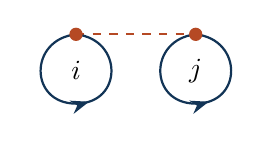
\begin{tikzpicture}[scale=1]
\draw[interaction] (-.95,0)--(.95,0);
\draw[fermion] (-.95,0)..controls(-1.7,-.08)and(-1.7,-1.1)..(-.95,-1.1)..controls(-.2,-1.1)and(-.2,-.08)..(-.95,0);
\draw[fermion] (.95,0)..controls(.2,-.08)and(.2,-1.1)..(.95,-1.1)..controls(1.7,-1.1)and(1.7,-.08)..(.95,0);
\node[vertex] at(-.95,0){};\node[vertex] at(.95,0){};
\node at(-.95,-.58){\(i\)};\node at(.95,-.58){\(j\)};
\end{tikzpicture}
\par\small Direct: \(+\tfrac12\sum_{ij}\langle ij|v|ij\rangle\).
\column{.48\textwidth}
\centering
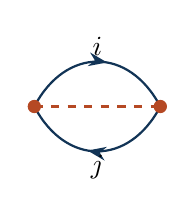
\begin{tikzpicture}[scale=1]
\draw[interaction] (-1,0)--(1,0);
\draw[fermion] (-1,0)..controls(-.5,.95)and(.5,.95)..(1,0);
\draw[fermion] (1,0)..controls(.5,-.95)and(-.5,-.95)..(-1,0);
\node[vertex]at(-1,0){};\node[vertex]at(1,0){};
\node at(0,.96){\(i\)};\node at(0,-.96){\(j\)};
\end{tikzpicture}
\par\small Exchange: \(-\tfrac12\sum_{ij}\langle ij|v|ji\rangle\).
\end{columns}
\medskip
\small Dashed line: two-body interaction. Solid loops: occupied-line contractions. The exchange sign is displayed explicitly in the algebra. Next week: the rules that produce the sign and the \(\tfrac12\) from the drawing.
\end{frame}

\begin{frame}{Which intermediate determinants contribute?}
\[
E^{(2)}=\sum_{m\ne0}
\frac{\mel{\ph}{H_I}{\Phi_m}\mel{\Phi_m}{H_I}{\ph}}
 {\varepsilon_0-\varepsilon_m}.
\]
For an interaction containing at most two-body operators,
\[
\ket{\ph}\xrightarrow{H_I}
\left\{\ket{\Phi_i^a},\ \ket{\Phi_{ij}^{ab}}\right\}
\xrightarrow{H_I}\ket{\ph}.
\]
\begin{block}{Two sectors at second order}
\[E^{(2)}=E^{(2)}_{1p1h}+E^{(2)}_{2p2h}.\]
\end{block}
\small A reference component is excluded by \(Q\). No triple or higher excitation can be reached from a determinant by a single two-body vertex.
\end{frame}

\begin{frame}{Normal ordering exposes the mean-field contraction}
For the partition just introduced (week 37, section 3.17),
\[
H=\Eref+F_N+V_N,
\qquad
F_N=\sum_{pq}(h^0_{pq}+U_{pq})\no{\cre{p}\ann{q}},
\]
\[
V_N=\frac14\sum_{pqrs}\vbar{p}{q}{r}{s}
\no{\cre{p}\cre{q}\ann{s}\ann{r}},
\qquad
\boxed{U_{pq}=\sum_{j\in\mathrm{occ}}\vbar{p}{j}{q}{j}.}
\]
\begin{itemize}
\item Braces denote normal ordering with respect to \(\ket{\ph}\).
\item \(U\) is the mean field called \(u^{\rm HF}\) in the notes.
\item This definition does not assume that the orbitals solve the HF equations.
\end{itemize}
\end{frame}

\begin{frame}{The interaction in normal-ordered form}
Since \(H_0=\sum_{pq}h^0_{pq}\cre{p}\ann{q}\) here,
\[
\boxed{H_I=V=E^{(1)}+U_N+V_N,}
\qquad
U_N=\sum_{pq}U_{pq}\no{\cre{p}\ann{q}},\qquad
V_N=\frac14\sum_{pqrs}\vbar{p}{q}{r}{s}
\no{\cre{p}\cre{q}\ann{s}\ann{r}}.
\]
\begin{itemize}
\item The scalar \(E^{(1)}\) cannot connect \(P\) and \(Q\).
\item \(U_N\) connects the reference to singles.
\item \(V_N\) connects the reference to doubles.
\end{itemize}
\warnbox{The braces matter: adding \(U_N\) to an un-normal-ordered bare two-body operator would count the mean-field contractions twice.}
\end{frame}

\begin{frame}{Evaluating the singles matrix element}
For \(\ket{\Phi_i^a}=\cre{a}\ann{i}\ket{\ph}\),
\[
\mel{\Phi_i^a}{\cre{p}\ann{q}}{\ph}
=\mel{\ph}{\cre{i}\ann{a}\cre{p}\ann{q}}{\ph}
=\delta_{pa}\delta_{qi}.
\]
The two nonzero contractions pair the occupied operators and the unoccupied operators:
\[
(\cre{i},\ann{q})\longrightarrow\delta_{iq},\qquad
(\ann{a},\cre{p})\longrightarrow\delta_{ap}.
\]
Therefore
\[
\boxed{\mel{\Phi_i^a}{H_I}{\ph}=U_{ai},\qquad
\mel{\ph}{H_I}{\Phi_i^a}=U_{ia}=U_{ai}^{*}.}
\]
\small Compare week 39: this is the Hartree-Fock matrix element \(\langle a|f|i\rangle\) with \(h_0\) diagonal.
\end{frame}

\begin{frame}{The singles contribution to the second-order energy}
The intermediate determinant has unperturbed energy
\(\varepsilon_i^a=\varepsilon_0-\varepsilon_i+\varepsilon_a\). Consequently,
\[
\boxed{E^{(2)}_{1p1h}=
\sum_{ia}\frac{U_{ia}U_{ai}}{\varepsilon_i-\varepsilon_a}
=\sum_{ia}\frac{|U_{ai}|^2}{\varepsilon_i-\varepsilon_a}.}
\]
Since \(U_{ai}=\sum_{j\in\mathrm{occ}}\vbar{a}{j}{i}{j}\),
\[
E^{(2)}_{1p1h}=
\sum_{ia}\frac{\left|\sum_{j\in\mathrm{occ}}\vbar{a}{j}{i}{j}\right|^2}
 {\varepsilon_i-\varepsilon_a}.
\]
\small The occupied-orbital contributions add before squaring. In general, \(\left|\sum_j z_j\right|^2\ne\sum_j|z_j|^2\).
\end{frame}

\begin{frame}{The leading singles amplitude and the CI energy}
When \(h_0\) is diagonal,
\[
\langle i\lvert h_0\rvert a\rangle=\varepsilon_a\braket{i}{a}=0,
\qquad f_{ia}=h^0_{ia}+U_{ia}=U_{ia}.
\]
The exact reference-projected singles energy is
\((E_0-\Eref)_{\rm singles}=\sum_{ia}c_i^a U_{ia}\).
Its leading perturbative approximation uses
\[
\boxed{c_i^{a(1)}=\frac{U_{ai}}{\varepsilon_i-\varepsilon_a},}
\qquad
\sum_{ia}c_i^{a(1)}U_{ia}
=\sum_{ia}\frac{|U_{ai}|^2}{\varepsilon_i-\varepsilon_a}.
\]
\mbbox{The exact amplitude \(c_i^a\) comes from the projected FCI equations of week 38; the perturbative amplitude is its leading term, and the second-order energy is the projected energy evaluated with it.}
\end{frame}

% ======================================================================
\section{Friday, lecture 3: Second order and a fourth-order check}
% ======================================================================

\begin{frame}{Connecting the CI energy and the perturbative expansion (section 9.5)}
For exact CI amplitudes,
\[
E_0-\Eref=\sum_{ia}c_i^a f_{ia}
+\frac14\sum_{ijab}c_{ij}^{ab}\vbar{i}{j}{a}{b}.
\]
Here and below, \(i,j,a,b\) are unrestricted within their occupied or unoccupied sets, and the doubles amplitudes are antisymmetric.
\[
E_0-\varepsilon_0=E^{(1)}+E^{(2)}+\cdots,
\qquad
E^{(2)}=\sum_{m\ne0}
\frac{\mel{\ph}{H_I}{\Phi_m}\mel{\Phi_m}{H_I}{\ph}}
 {\varepsilon_0-\varepsilon_m}.
\]
\small The perturbative amplitudes approximate the exact configuration amplitudes. The energy baseline remains \(\Eref=\varepsilon_0+E^{(1)}\).
\end{frame}

\begin{frame}{Singles: the coherent mean-field sum}
For the diagonal-\(h_0\), bare-interaction partition,
\[
f_{ia}=U_{ia},\qquad U_{ai}=\sum_{j\in\mathrm{occ}}\vbar{a}{j}{i}{j},\qquad
c_i^{a(1)}=\frac{U_{ai}}{\varepsilon_i-\varepsilon_a}.
\]
Then
\[
E^{(2)}_{1p1h}
=\sum_{ia}\frac{U_{ia}U_{ai}}{\varepsilon_i-\varepsilon_a}
=\sum_{ia}\sum_{jk\in\mathrm{occ}}
\frac{\vbar{i}{j}{a}{j}\vbar{a}{k}{i}{k}}
 {\varepsilon_i-\varepsilon_a}.
\]
\begin{exampleblock}{Keep the cross terms}
The \(j\) and \(k\) sums are independent: this is the modulus squared of a sum over occupied orbitals, not the sum of individual moduli squared.
\end{exampleblock}
\end{frame}

\begin{frame}{Pause to think \#3}
\thinkq{3}{The singles term \(E^{(2)}_{1p1h}=\sum_{ia}|\sum_jv_{ajij}|^2/(\varepsilon_i-\varepsilon_a)\) is a double sum over occupied \(j,k\).
\begin{enumerate}
\item For the pairing model (levels \(p\), spins \(\pm\), interaction moving pairs only), what is \(U_{ai}\)? What is \(E^{(2)}_{1p1h}\)?
\item For the pairing plus particle-hole model of week 39 the answer is different. Why?
\item What happens to this term in a Hartree-Fock basis -- and what does the mean field have to be for that to happen?
\end{enumerate}}
\end{frame}

\begin{frame}{Answer to pause \#3}
\thinka{%
\begin{enumerate}
\item The pairing interaction \(\vbar{a}{j}{i}{j}\) needs \(a\) and \(i\) to be the two members of the same pair, which is impossible for \(a\) empty and \(i\) occupied in the reference: \(U_{ai}=0\), and the singles term vanishes identically, for every \(g\) and every basis.
\item The particle-hole term breaks pairs and connects \(\ket{\ph}\) to \(1p1h\) states, so \(U_{ai}\ne0\); its value is a coherent sum over the two occupied levels, and the squared sum is what the week-45 table will list as \(E^{(2)}_{1p1h}\).
\item \(f_{ai}=0\) by Brillouin's theorem: the HF mean field \(u^{\rm HF}\) is exactly the \(U\) defined here, evaluated in the self-consistent orbitals, so the whole \(1p1h\) sector disappears at second order -- which is the practical reason to build perturbation theory on a Hartree-Fock reference.
\end{enumerate}}
\end{frame}

\begin{frame}{Doubles: two interaction vertices before contraction}
For a double-excitation intermediate state, use
\[
A_{pqrs}=\cre{p}\cre{q}\ann{s}\ann{r},\qquad
V=\frac14\sum_{pqrs}\vbar{p}{q}{r}{s}A_{pqrs}.
\]
The doubles sector is
\[
E^{(2)}_{2p2h}
=\frac1{16}\sum_{m\in2p2h}\sum_{pqrs}\sum_{tuvw}
\frac{\vbar{p}{q}{r}{s}\vbar{t}{u}{v}{w}}
 {\varepsilon_0-\varepsilon_m}
\,\mel{\ph}{A_{pqrs}}{\Phi_m}
\mel{\Phi_m}{A_{tuvw}}{\ph}.
\]
\begin{itemize}
\item Each vertex contributes a factor \(1/4\), hence \(1/16\) before contractions.
\item In this formula, each intermediate determinant \(m\) is counted once.
\end{itemize}
\end{frame}

\begin{frame}{Wick contractions and antisymmetry}
Evaluate
\(\mel{\ph}{\cre{p}\cre{q}\ann{s}\ann{r}\cre{a}\cre{b}\ann{j}\ann{i}}{\ph}\):
\begin{columns}[T,onlytextwidth]
\column{.49\textwidth}\centering
\wickpattern{1}
\[
+\delta_{pi}\delta_{qj}\delta_{ra}\delta_{sb}
\quad\Rightarrow\quad +\vbar{i}{j}{a}{b}.
\]
\column{.49\textwidth}\centering
\wickpattern{2}
\[
-\delta_{pi}\delta_{qj}\delta_{rb}\delta_{sa}
\quad\Rightarrow\quad -\vbar{i}{j}{b}{a}=+\vbar{i}{j}{a}{b}.
\]
\end{columns}
\medskip
\small Exchanging the occupied contractions gives two more equivalent terms. Together, four contractions cancel the \(1/4\) at a vertex:
\[
\boxed{\mel{\ph}{V}{\Phi_{ij}^{ab}}=\vbar{i}{j}{a}{b}.}
\]
\end{frame}

\begin{frame}{The doubles denominator and the counting factor}
The unperturbed double excitation has energy
\(\varepsilon_{ij}^{ab}=\varepsilon_0+\varepsilon_a+\varepsilon_b-\varepsilon_i-\varepsilon_j\).
An unrestricted index sum counts each determinant four times:
\[
Q_{2p2h}=\sum_{\substack{i<j\\a<b}}
\ket{\Phi_{ij}^{ab}}\bra{\Phi_{ij}^{ab}}
=\frac14\sum_{ijab}\ket{\Phi_{ij}^{ab}}\bra{\Phi_{ij}^{ab}}.
\]
Therefore
\[
\boxed{E^{(2)}_{2p2h}=\frac14\sum_{ijab}
\frac{\vbar{i}{j}{a}{b}\vbar{a}{b}{i}{j}}
 {\varepsilon_i+\varepsilon_j-\varepsilon_a-\varepsilon_b}.}
\]
\small For Hermitian \(V\), the numerator is \(|\vbar{a}{b}{i}{j}|^2\). With \(i<j\) and \(a<b\), omit the factor \(1/4\).
\end{frame}

\begin{frame}{Pause to think \#4}
\thinkq{3}{Factors of two and four.
\begin{enumerate}
\item The vertex carries \(\tfrac14\) and the four Wick contractions cancel it. The sum over intermediate determinants carries another \(\tfrac14\) if the indices are unrestricted. Which \(\tfrac14\) survives in \(E^{(2)}_{2p2h}\), and why?
\item For the pairing model with four levels and two pairs, how many double excitations are there, and what is \(E^{(2)}\) in terms of \(g\)? (Week 38: the first iterate of the FCI equations.)
\end{enumerate}}
\end{frame}

\begin{frame}{Answer to pause \#4}
\thinka{%
\begin{enumerate}
\item The vertex \(\tfrac14\) is cancelled by the four ways of contracting \(\cre{p}\cre{q}\ann{s}\ann{r}\) with the excitation, which all give the same antisymmetrised element -- that is what antisymmetrised elements are for. The counting \(\tfrac14\) survives only if one \emph{chooses} to sum over all \(i,j,a,b\); with \(i<j\), \(a<b\) each determinant appears once and there is no factor. The two conventions give the same number; mixing them gives a factor four.
\item Four: each of the two occupied pairs lifted to each of the two empty levels, matrix element \(-g/2\), denominator \(2(\varepsilon_i-\varepsilon_a)\in\{-2,-4,-4,-6\}\) for unit spacing: \(E^{(2)}=\frac{g^2}{4}\left(-\frac12-\frac14-\frac14-\frac16\right)=-\frac{7}{24}g^2\), the first iterate of the projected equations of week 38.
\end{enumerate}}
\end{frame}

\begin{frame}{The leading doubles amplitude}
The first-order state correction contains
\(\ket{\Psi_0^{(1)}}=R_0H_I\ket{\ph}\).
Projecting onto a double excitation gives
\[
\boxed{c_{ij}^{ab(1)}=
\frac{\mel{\Phi_{ij}^{ab}}{H_I}{\ph}}
 {\varepsilon_0-\varepsilon_{ij}^{ab}}
=\frac{\vbar{a}{b}{i}{j}}
 {\varepsilon_i+\varepsilon_j-\varepsilon_a-\varepsilon_b}.}
\]
The corresponding CI energy contribution becomes
\[
\frac14\sum_{ijab}c_{ij}^{ab(1)}\vbar{i}{j}{a}{b}
=E^{(2)}_{2p2h}.
\]
\small A first-order wave-function amplitude enters the second-order energy. Excitation rank and perturbative order are different labels.
\end{frame}

\begin{frame}{The complete second-order energy}
For the bare-interaction partition with diagonal \(h_0\),
\[
\boxed{\begin{aligned}
E^{(2)}={}&\sum_{ia}\frac{|U_{ai}|^2}{\varepsilon_i-\varepsilon_a}
+\frac14\sum_{ijab}
\frac{|\vbar{a}{b}{i}{j}|^2}
 {\varepsilon_i+\varepsilon_j-\varepsilon_a-\varepsilon_b},
\end{aligned}}
\qquad
E_0^{[2]}=\Eref+E^{(2)},\qquad
U_{ai}=\sum_{j\in\mathrm{occ}}\vbar{a}{j}{i}{j}.
\]
\begin{exampleblock}{Canonical HF specialisation}
In the usual HF-based partition, the residual reference-to-single coupling vanishes. Only the doubles term remains (M\o{}ller-Plesset second order, MP2). Changing the partition also changes the unperturbed energies and the residual operator.
\end{exampleblock}
\end{frame}

\begin{frame}{A variant benchmark: purely off-diagonal coupling (section 9.5)}
Now remove the diagonal interaction present in the earlier example:
\[
H=H_0+V,\qquad H_0=\sum_{p=1}^{2}\varepsilon_p\cre{p}\ann{p},
\qquad V=\lambda\sum_{p\ne q}\cre{p}\ann{q}.
\]
\begin{columns}[c,onlytextwidth]
\column{.38\textwidth}\centering
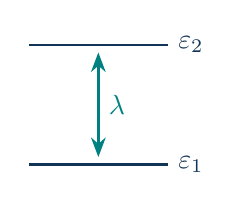
\begin{tikzpicture}[scale=1]
\draw[uioblue,line width=1pt](-1.1,0)--(1.1,0)node[right]{\(\varepsilon_1\)};
\draw[uioblue,line width=1pt](-1.1,1.9)--(1.1,1.9)node[right]{\(\varepsilon_2\)};
\draw[teal,{Stealth}-{Stealth},line width=.9pt](0,.12)--(0,1.78)node[midway,right]{\(\lambda\)};
\end{tikzpicture}
\column{.58\textwidth}
\[
H=\begin{pmatrix}\varepsilon_1&\lambda\\\lambda&\varepsilon_2\end{pmatrix},
\qquad \varepsilon_1<\varepsilon_2,
\]
\[
V_{11}=V_{22}=0,\quad V_{12}=V_{21}=\lambda.
\]
\small One-particle basis: \(\ket{\Phi_1}=\cre{1}\ket{0}\), \(\ket{\Phi_2}=\cre{2}\ket{0}\).
\end{columns}
\vspace{0.5em}
The lower eigenvalue, with \(\Delta=\varepsilon_2-\varepsilon_1>0\):
\[
\boxed{E_-=
\frac{\varepsilon_1+\varepsilon_2}{2}
-\frac12\sqrt{\Delta^2+4\lambda^2}
=\varepsilon_1+\frac\Delta2
\left[1-\sqrt{1+\frac{4\lambda^2}{\Delta^2}}\right].}
\]
\end{frame}

\begin{frame}{Brillouin-Wigner: a two-vertex equation is exact here}
Choose \(P=\ket{\Phi_1}\bra{\Phi_1}\) and \(Q=\ket{\Phi_2}\bra{\Phi_2}\).
Because \(V_{11}=V_{22}=0\), all further \(Q\)-space interaction insertions vanish:
\[
QVQ=0,\qquad
\boxed{E_--\varepsilon_1=\frac{\lambda^2}{E_--\varepsilon_2},}
\qquad
\boxed{(E_--\varepsilon_1)(E_--\varepsilon_2)-\lambda^2=0,}
\]
which is the exact secular equation.
\begin{block}{An important qualification}
The energy-dependent equation is solved self-consistently. Its solution contains all even powers of \(\lambda\), despite having only two explicit vertices. In this particular two-state model the BW solution is exact; this property does not hold for a generic two-vertex truncation (chapter 9: BW(2) and BW(3) for the pairing model are well off).
\end{block}
\end{frame}

\begin{frame}{The same virtual excursion in two representations}
\[
1\xrightarrow{\lambda}2\xrightarrow{\lambda}1,
\qquad \frac{V_{12}V_{21}}{E_--\varepsilon_2}
=\frac{\lambda^2}{E_--\varepsilon_2}.
\]
\begin{columns}[c,onlytextwidth]
\column{.47\textwidth}\centering
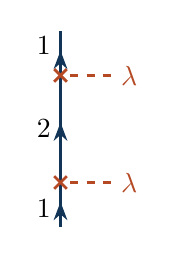
\begin{tikzpicture}[scale=1]
\draw[fermion](0,-.7)--(0,0);
\draw[fermion](0,0)--(0,1.7);
\draw[fermion](0,1.7)--(0,2.4);
\foreach \y in {0,1.7}{\draw[warm,line width=1pt](-.1,\y-.1)--(.1,\y+.1);\draw[warm,line width=1pt](-.1,\y+.1)--(.1,\y-.1);\draw[interaction](.15,\y)--(.8,\y)node[right]{\(\lambda\)};}
\node[left]at(0,-.42){\(1\)};\node[left]at(0,.85){\(2\)};\node[left]at(0,2.17){\(1\)};
\end{tikzpicture}
\par\small One-body transition chain.
\column{.47\textwidth}\centering
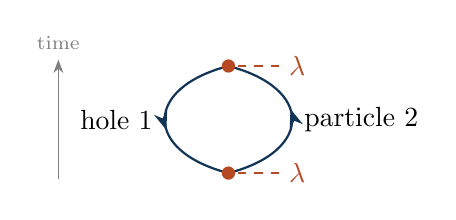
\begin{tikzpicture}[scale=1]
\draw[fermion](0,0)..controls(1.35,.35)and(1.35,1.35)..(0,1.7);
\draw[fermion](0,1.7)..controls(-1.35,1.35)and(-1.35,.35)..(0,0);
\foreach \y in {0,1.7}{\node[vertex]at(0,\y){};\draw[interaction](.15,\y)--(.8,\y)node[right]{\(\lambda\)};}
\node[right]at(1.05,.85){particle \(2\)};
\node[left]at(-1.05,.85){hole \(1\)};
\draw[-{Stealth},gray](-2.7,-.1)--(-2.7,1.8)node[above]{\scriptsize time};
\end{tikzpicture}
\par\small Closed particle-hole representation.
\end{columns}
\medskip
\small Next week turns the right-hand picture into a rule: a cut between the two vertices gives the denominator, the loop gives the sign.
\end{frame}

\begin{frame}{Rayleigh-Schr\"odinger terms through third order}
Write \(D=\varepsilon_1-\varepsilon_2<0\). The denominators are now fixed:
\[
E^{(1)}=V_{11}=0,\qquad
\boxed{E^{(2)}=\frac{V_{12}V_{21}}{D}=\frac{\lambda^2}{D}.}
\qquad
E^{(3)}=\frac{V_{12}V_{22}V_{21}}{D^2}
-\frac{V_{11}V_{12}V_{21}}{D^2}=0.
\]
Therefore the total energy through third order is
\[
\boxed{E_-^{[3]}=\varepsilon_1+\frac{\lambda^2}{D}.}
\]
\small The third-order coefficient vanishes; the sum through third order still contains the nonzero second-order term.
\end{frame}

\begin{frame}{Fixed and self-consistent denominators differ at finite order}
\begin{columns}[T,onlytextwidth]
\column{.48\textwidth}
\begin{block}{RS through third order}
\[
\Delta E^{[3]}=\frac{\lambda^2}{D}.
\]
One fixed unperturbed energy denominator.
\end{block}
\column{.48\textwidth}
\begin{exampleblock}{Self-consistent BW}
\[
\Delta E^{\rm BW}=\frac{\lambda^2}{D+\Delta E^{\rm BW}}.
\]
The denominator contains the correlated energy shift.
\end{exampleblock}
\end{columns}
\medskip
Both start with \(\lambda^2/D\), but the BW solution also contains higher even powers. Thus
\(\Delta E^{[3]}\ne\Delta E^{\rm BW}\) for finite nonzero \(\lambda\).
\small In this particular two-state model the BW solution is exact; this property does not hold for a generic two-vertex truncation.
\end{frame}

\begin{frame}{The exact expansion identifies the fourth-order target}
Using \(D=\varepsilon_1-\varepsilon_2<0\), expand the exact square root:
\[
\boxed{E_-=\varepsilon_1+\frac{\lambda^2}{D}
\left[1-\frac{\lambda^2}{D^2}+\cdots\right].}
\qquad
\boxed{E^{(4)}=-\frac{\lambda^4}{D^3}>0.}
\]
\begin{itemize}
\item The Taylor expansion about \(\lambda=0\) applies inside \(|2\lambda/\Delta|<1\).
\item Low-order accuracy requires the coupling to be small relative to the gap.
\item The exact square-root expression remains defined outside this expansion region.
\end{itemize}
\end{frame}

\begin{frame}{Fourth-order RS terms in resolvent form}
For this benchmark only, set
\[
\av{X}=\mel{\Phi_1}{X}{\Phi_1},\qquad
R=\frac{Q}{\varepsilon_1-H_0},\qquad Q=\ket{\Phi_2}\bra{\Phi_2}.
\]
The fourth-order expression is
\begin{align*}
E^{(4)}={}&\av{VRVRVRV}
-E^{(1)}\left[\av{VR^2VRV}+\av{VRVR^2V}\right]
+\bigl(E^{(1)}\bigr)^2\av{VR^3V}
-E^{(2)}\av{VR^2V}.
\end{align*}
\begin{itemize}
\item \(E^{(1)}=V_{11}=0\) removes the middle terms.
\item \(QVQ=0\) removes the first term.
\item Only the final normalisation (folded) term survives.
\end{itemize}
\end{frame}

\begin{frame}{The surviving fourth-order term}
Since \(R=\ket{\Phi_2}\bra{\Phi_2}/D\),
\[
E^{(2)}=\av{VRV}=\frac{\lambda^2}{D},\qquad
\av{VR^2V}=\frac{\lambda^2}{D^2},
\qquad
\boxed{E^{(4)}=-E^{(2)}\av{VR^2V}
=-\frac{\lambda^4}{D^3},\qquad D<0.}
\]
\begin{exampleblock}{Agreement with the exact lower eigenvalue}
\[
E_-=\varepsilon_1+
\frac{\lambda^2}{\varepsilon_1-\varepsilon_2}
-\frac{\lambda^4}{(\varepsilon_1-\varepsilon_2)^3}
+\ord{\lambda^6}.
\]
\end{exampleblock}
\small The second-order shift is negative; the fourth-order correction is positive. A reader who drops the ``normalisation corrections'' gets the fourth order of this problem not approximately but completely wrong: there is nothing else.
\end{frame}

\begin{frame}{Pause to think \#5}
\thinkq{3}{The exact eigenvalue \(E_-(\lambda)\) is a smooth function of \(\lambda\) on the whole real axis, yet its Taylor series converges only for \(|2\lambda/\Delta|<1\).
\begin{enumerate}
\item Where are the singularities of \(E_-(\lambda)\) that limit the radius? Are they ever visited by a real calculation?
\item At \(\lambda/\Delta=0.55\) the terms \(|E^{(n)}|\) decrease for fifteen orders before they start to grow. What would a calculation stopped at fourth order conclude?
\end{enumerate}}
\end{frame}

\begin{frame}{Answer to pause \#5}
\thinka{%
\begin{enumerate}
\item At the branch points of the square root, \(4\lambda^2=-\Delta^2\), i.e.\ \(\lambda=\pm i\Delta/2\): complex couplings, never visited, but they fix the radius of convergence about \(\lambda=0\) all the same.
\item That the series converges. Nothing in the first few orders announces the radius; the terms simply stop decreasing much later. Chapter 9 finds the same behaviour in the pairing model beyond \(g\approx1.5\), where no closed form says where the singularity sits.
\end{enumerate}}
\end{frame}

\begin{frame}{The benchmark drawn: partial sums and terms}
  \centering
  \includegraphics[width=0.92\textwidth]{chapter09/mbpt_fig01}
  \par\small Left: exact \(E_-\) and RS partial sums through orders 2, 4, 8, 16 against \(\lambda/\Delta\); the dotted line is the radius \(\lambda/\Delta=\tfrac12\). Right: \(|E^{(n)}|\) for \(\lambda/\Delta=0.3,0.45,0.55,0.7\) -- geometric decrease inside, eventual growth outside, from the sixth order at \(0.7\) and only from the sixteenth at \(0.55\). (\texttt{mbpt.py}, chapter 9, section 9.5.)
\end{frame}

% ======================================================================
\section{Friday, lecture 4: All contributions, listed}
% ======================================================================

\begin{frame}{The recursion that generates every order}
With \(R_0=Q/(\varepsilon_0-H_0)\) and \(\ket{\Psizero}=\sum_n\ket{\Psi^{(n)}}\), \(\ket{\Psi^{(0)}}=\ket{\ph}\), collecting powers of \(\eta\) in \(\ket{\Psizero}=\ket{\ph}+R_0(H_I-\Delta E)\ket{\Psizero}\) gives
\[
\boxed{\ket{\Psi^{(n)}}=R_0\Bigl[H_I\ket{\Psi^{(n-1)}}-\sum_{k=1}^{n-1}E^{(k)}\ket{\Psi^{(n-k)}}\Bigr],
\qquad
E^{(n+1)}=\mel{\ph}{H_I}{\Psi^{(n)}}.}
\]
\begin{itemize}
\item The subtracted terms are the normalisation (``renormalisation'', ``unlinked'') corrections; they appear from \(n=2\) on.
\item \(R_0\ket{\ph}=0\): every \(\ket{\Psi^{(n)}}\), \(n\ge1\), lies in \(Q\) space, so intermediate normalisation is preserved order by order.
\item \texttt{mbpt.py} implements exactly this recursion and checks it against the explicit expressions on the next two frames.
\end{itemize}
\end{frame}

\begin{frame}[shrink=5]{All contributions to the wave operator through third order}
Write \(\ket{\Psizero}=\Omega\ket{\ph}\) with \(\Omega=1+\Omega^{(1)}+\Omega^{(2)}+\Omega^{(3)}+\cdots\), \(R\equiv R_0\), \(V\equiv H_I\):
\begin{align*}
\Omega^{(1)}&=RV,\\[2pt]
\Omega^{(2)}&=RVRV\;-\;E^{(1)}R^2V,\\[2pt]
\Omega^{(3)}&=RVRVRV\;-\;E^{(1)}\bigl[RVR^2V+R^2VRV\bigr]\;+\;\bigl(E^{(1)}\bigr)^2R^3V\;-\;E^{(2)}R^2V .
\end{align*}
In the determinant basis, with \(V_{mn}=\mel{\Phi_m}{H_I}{\Phi_n}\) and \(D_m=\varepsilon_0-\varepsilon_m\) (\(m,n,l\ne0\)):
\begin{align*}
\langle\Phi_m|\Psi^{(1)}\rangle&=\frac{V_{m0}}{D_m},\qquad
\langle\Phi_m|\Psi^{(2)}\rangle=\sum_{n}\frac{V_{mn}V_{n0}}{D_mD_n}-\frac{V_{00}V_{m0}}{D_m^2},\\
\langle\Phi_m|\Psi^{(3)}\rangle&=\sum_{nl}\frac{V_{mn}V_{nl}V_{l0}}{D_mD_nD_l}
-V_{00}\Bigl[\sum_n\frac{V_{mn}V_{n0}}{D_mD_n^2}+\sum_n\frac{V_{mn}V_{n0}}{D_m^2D_n}\Bigr]
+V_{00}^2\frac{V_{m0}}{D_m^3}
-E^{(2)}\frac{V_{m0}}{D_m^2}.
\end{align*}
\small For a two-body \(H_I\): \(\Psi^{(1)}\) has singles (\(U_{ai}/(\varepsilon_i-\varepsilon_a)\)) and doubles (\(\vbar{a}{b}{i}{j}/(\varepsilon_i+\varepsilon_j-\varepsilon_a-\varepsilon_b)\)); \(\Psi^{(2)}\) reaches up to quadruples; \(\Psi^{(3)}\) up to sextuples. Rank is not order.
\end{frame}

\begin{frame}[shrink=5]{All contributions to the energy through fourth order}
With \(\av{X}=\mel{\ph}{X}{\ph}\), \(R=Q/(\varepsilon_0-H_0)\), \(V=H_I\), and \(E^{(n+1)}=\av{V\Omega^{(n)}}\):
\begin{align*}
E^{(1)}&=\av{V},\\[2pt]
E^{(2)}&=\av{VRV},\\[2pt]
E^{(3)}&=\av{VRVRV}\;-\;E^{(1)}\av{VR^2V},\\[2pt]
E^{(4)}&=\av{VRVRVRV}\;-\;E^{(1)}\bigl[\av{VR^2VRV}+\av{VRVR^2V}\bigr]\;+\;\bigl(E^{(1)}\bigr)^2\av{VR^3V}\;-\;E^{(2)}\av{VR^2V}.
\end{align*}
In the determinant basis:
\begin{align*}
E^{(1)}&=V_{00},\qquad E^{(2)}=\sum_m\frac{V_{0m}V_{m0}}{D_m},\qquad
E^{(3)}=\sum_{mn}\frac{V_{0m}V_{mn}V_{n0}}{D_mD_n}-V_{00}\sum_m\frac{V_{0m}V_{m0}}{D_m^2},\\
E^{(4)}&=\sum_{mnl}\frac{V_{0m}V_{mn}V_{nl}V_{l0}}{D_mD_nD_l}
-2V_{00}\sum_{mn}\frac{V_{0m}V_{mn}V_{n0}}{D_m^2D_n}
+V_{00}^2\sum_m\frac{V_{0m}V_{m0}}{D_m^3}
-\Bigl(\sum_n\frac{V_{0n}V_{n0}}{D_n}\Bigr)\sum_m\frac{V_{0m}V_{m0}}{D_m^2}.
\end{align*}
\small (The two mixed terms are complex conjugates, equal for real matrix elements, hence the \(2\).) Every term with a factor \(E^{(k)}\) in front is a renormalisation term: the product of two separately evaluated pieces. Next week: these are the \emph{unlinked} diagrams, and they cancel against the unlinked parts of the principal term -- the linked-diagram theorem.
\end{frame}

\begin{frame}{The same list in the language of determinants, through second order}
For \(H_0=\sum_p\varepsilon_p\cre{p}\ann{p}\) and \(H_I=E^{(1)}+U_N+V_N\):
\begin{align*}
E^{(1)}&=\sum_{i}u_{ii}+\frac12\sum_{ij\in\mathrm{occ}}\vbar{i}{j}{i}{j}
\quad(\text{with } u=0 \text{ for a diagonal } h_0),\\[2pt]
E^{(2)}&=\underbrace{\sum_{ia}\frac{|U_{ai}|^2}{\varepsilon_i-\varepsilon_a}}_{1p1h}
+\underbrace{\frac14\sum_{ijab}\frac{|\vbar{a}{b}{i}{j}|^2}{\varepsilon_i+\varepsilon_j-\varepsilon_a-\varepsilon_b}}_{2p2h},\\[2pt]
\Omega^{(1)}\ket{\ph}&=\sum_{ia}\frac{U_{ai}}{\varepsilon_i-\varepsilon_a}\ket{\Phi_i^a}
+\frac14\sum_{ijab}\frac{\vbar{a}{b}{i}{j}}{\varepsilon_i+\varepsilon_j-\varepsilon_a-\varepsilon_b}\ket{\Phi_{ij}^{ab}}.
\end{align*}
\numbox{Four models, \texttt{mbpt.py}: the fourth order from the explicit formula and from the recursion agree to \(10^{-12}\). Hubbard (\(U=2\)): the four pieces are \(-0.191\), \(+0.303\), \(-0.151\), \(+0.032\) and the total \(-0.0076\). The cancellations are severe, and they are the point of next week.}
\end{frame}

\begin{frame}{Pause to think \#6}
\thinkq{3}{Look at the list of fourth-order terms.
\begin{enumerate}
\item How many distinct terms does \(E^{(4)}\) have for a reference with \(E^{(1)}=0\) (Hartree-Fock partition with the mean field in \(H_0\))?
\item In the third order, \(E^{(1)}\av{VR^2V}\) is the product of two quantities that are each sums over the whole system. If the system were two non-interacting copies of a smaller one, how would this product scale with the number of copies? And \(E^{(3)}\) itself?
\end{enumerate}}
\end{frame}

\begin{frame}{Answer to pause \#6}
\thinka{%
\begin{enumerate}
\item Two: the principal term \(\av{VRVRVRV}\) and the folded term \(-E^{(2)}\av{VR^2V}\). For the Lipkin model (\(E^{(1)}=0\)) \texttt{mbpt.py} gives \(-0.0036\) and \(+0.0072\), total \(+0.0036\).
\item \(E^{(1)}\) and \(\av{VR^2V}\) each scale linearly with the number of copies, so their product scales \emph{quadratically} -- an energy cannot. The principal term \(\av{VRVRV}\) contains a quadratically scaling piece of its own, and the subtraction removes it exactly: \(E^{(3)}\) scales linearly. This is size extensivity, verified to machine precision in chapter 9, and next week it becomes the statement that only \emph{linked} diagrams contribute.
\end{enumerate}}
\end{frame}

% ======================================================================
\section{Summary}
% ======================================================================

\begin{frame}{Summary of week 44}
  \small
  \begin{columns}[T]
    \column{0.48\textwidth}
    \begin{block}{Thursday: the framework}
      \begin{itemize}
        \item \(E_0-\Eref=\sum c_i^af_{ia}+\sum c_{ij}^{ab}\vbar{i}{j}{a}{b}\): singles and doubles couple directly
        \item Intermediate normalisation; \(\Delta E=E_0-\varepsilon_0\) versus \(E_0-\Eref\)
        \item \(P\), \(Q\), the reduced resolvent, an exact equation, its Neumann series
        \item BW: \(\omega=E_0\), implicit, resummed into \(G_Q\) and \(H_{\rm eff}(E_0)\), exact for the two-state model
        \item RS: \(\omega=\varepsilon_0\), \(E^{(1)}=\av{H_I}\), \(E^{(2)}=\av{H_IR_0H_I}\), \(E^{(3)}\) with its normalisation subtraction
      \end{itemize}
    \end{block}
    \column{0.48\textwidth}
    \begin{block}{Friday: the terms}
      \begin{itemize}
        \item \(H_I=E^{(1)}+U_N+V_N\) with \(U_{pq}=\sum_j\vbar{p}{j}{q}{j}\): singles from \(U_N\), doubles from \(V_N\)
        \item \(E^{(2)}=\sum|U_{ai}|^2/(\varepsilon_i-\varepsilon_a)+\frac14\sum|\vbar{a}{b}{i}{j}|^2/(\ldots)\): coherent sum, four contractions, counting factor
        \item Two-level benchmark: BW exact with two vertices; RS \(E^{(3)}=0\), \(E^{(4)}=-E^{(2)}\av{VR^2V}\); radius \(|2\lambda/\Delta|=1\)
        \item The complete lists: \(\Omega^{(1,2,3)}\) and \(E^{(1,2,3,4)}\)
      \end{itemize}
    \end{block}
  \end{columns}
  \vspace{0.3em}
  \centering The renormalisation terms are not corrections: they cancel exactly what would make the energy scale wrongly with system size.
\end{frame}

\begin{frame}{Next week}
  \begin{exampleblock}{Week 45, November 5--6: diagram rules and their derivation (chapter 9, sections 9.6--9.12)}
    \small
    Every term listed today is drawn: the perturbation as a cross (one-body remainder) and a dashed line (interaction), particle and hole lines, the reference as the vacuum, and the \emph{energy denominator} as a cut between successive vertices. The rules -- sums over labels, a denominator per cut, \(\tfrac12\) per pair of equivalent lines, the sign \((-1)^{h+l}\) -- are derived from Wick's theorem, and the first-order, first-order-wave-function and second-order diagrams are read off and matched to today's formulas. Then third order, the unlinked diagrams, and the linked-diagram theorem: why the renormalisation terms exist and what they cancel. Numerics: the four models of chapter 9 order by order, size extensivity, and how far the series can be trusted.
  \end{exampleblock}
  \vspace{0.5em}
  \small
  Reading: chapter 9, sections 9.6--9.12; Shavitt and Bartlett, chapters 4--5. The week-44 exercises (next two frames, \texttt{Exercises/ExercisesWeek44.tex}) are discussed in the exercise session and answered on the week-45 slides.
\end{frame}

% ======================================================================
\section{Exercises, week 44}
% ======================================================================

\begin{frame}[shrink=5]{Exercise 1: the expansion from the projected equation}
Let \(H=H_0+V\) and \(\ket{\phi_n}\) be the eigenstates of \(H_0\) and \(\ket{\psi_n}\) the corresponding ones for \(H\). Assume that the ground states \(\ket{\phi_0}\) and \(\ket{\psi_0}\) are not degenerate. Show that
\[
E_0-\varepsilon_0=\frac{\bra{\phi_0}V\ket{\psi_0}}{\braket{\phi_0}{\psi_0}},
\qquad
H\ket{\psi_0}=E_0\ket{\psi_0},\qquad H_0\ket{\phi_0}=\varepsilon_0\ket{\phi_0}.
\]
\begin{enumerate}
\item[a)] Define the operators \(P=\ket{\phi_0}\bra{\phi_0}\) and \(Q=1-P\). Show that these operators are idempotent.
\item[b)] Show that for any \(z\) we have
\begin{align*}
\ket{\psi_0}&=\braket{\phi_0}{\psi_0}\sum_{n=0}^{\infty}\left(\frac{Q}{z-H_0}(z-E_0+V)\right)^n\ket{\phi_0},\\
E_0&=\varepsilon_0+\sum_{n=0}^{\infty}\bra{\phi_0}V\left(\frac{Q}{z-H_0}(z-E_0+V)\right)^n\ket{\phi_0}.
\end{align*}
\item[c)] Discuss these results for \(z=E_0\) (Brillouin-Wigner perturbation theory) and \(z=\varepsilon_0\) (Rayleigh-Schr\"odinger perturbation theory). Compare the first few terms in these expansions.
\end{enumerate}
\small Note the overlap \(\braket{\phi_0}{\psi_0}\) in the denominator: this is the general form, before intermediate normalisation sets it to one.
\end{frame}

\begin{frame}[shrink=4]{Exercise 2: two particles in a single \(j\)-shell}
Consider a system of two fermions with spin \(s=1/2\) in the pair-orbitals \(\ket{m_0}\) and \(\ket{-m_0}\) in a single shell \(j=l+s\) with \(2j+1>2\), where \(l\) is the orbital momentum with \(l=0,1,2,\dots\). Assume that the matrix elements for the interaction between the particles take the form
\[
\bra{m,-m}v\ket{m',-m'}=-G .
\]
\begin{enumerate}
\item[a)] Show that the Brillouin-Wigner expansion from the previous exercise can be used to give
\[
E_0=-(j+1/2)G .
\]
\item[b)] Show thereafter by direct diagonalisation of the Hamiltonian matrix that this is the exact energy. Use thereafter Rayleigh-Schr\"odinger perturbation theory and discuss the differences.
\end{enumerate}
\mbbox{Hint for the discussion in b): all \(j+1/2\) pair states are degenerate in \(H_0\). Which of the two schemes survives that, and why? (Today's reduced resolvent is the place to look.)}
\end{frame}

\end{document}
